\documentclass{tufte-handout}

%\title{An Example of the Usage of the Tufte-Handout Style\thanks{Inspired by Edward~R. Tufte!}}
\title{Two-Class Classification Task\thanks{CS-GY-6923\newline Course Instructor: Gang Li;\newline TA: Xu Zhao}}
%\author[The Tufte-LaTeX Developers]{The Tufte-\LaTeX\ Developers}
\author[Yun Yan]{Yun Yan (\href{mailto:yy1533@nyu.edu}{yy1533@nyu.edu})}
\date{Oct 20, 2015} % without \date command, current date is supplied

%\geometry{showframe} % display margins for debugging page layout

\usepackage{graphicx} % allow embedded images
  \setkeys{Gin}{width=\linewidth,totalheight=\textheight,keepaspectratio}
  \graphicspath{{/Users/yunyan/Yun_Codes/Git_Public_Pres_and_Blog/ML_course_Project/fig/}} % set of paths to search for images
\usepackage{amsmath}  % extended mathematics
\usepackage{booktabs} % book-quality tables
\usepackage{units}    % non-stacked fractions and better unit spacing
\usepackage{multicol} % multiple column layout facilities
\usepackage{lipsum}   % filler text
\usepackage{fancyvrb} % extended verbatim environments
  \fvset{fontsize=\normalsize}% default font size for fancy-verbatim environments

% Standardize command font styles and environments
\newcommand{\doccmd}[1]{\texttt{\textbackslash#1}}% command name -- adds backslash automatically
\newcommand{\docopt}[1]{\ensuremath{\langle}\textrm{\textit{#1}}\ensuremath{\rangle}}% optional command argument
\newcommand{\docarg}[1]{\textrm{\textit{#1}}}% (required) command argument
\newcommand{\docenv}[1]{\textsf{#1}}% environment name
\newcommand{\docpkg}[1]{\texttt{#1}}% package name
\newcommand{\doccls}[1]{\texttt{#1}}% document class name
\newcommand{\docclsopt}[1]{\texttt{#1}}% document class option name
\newenvironment{docspec}{\begin{quote}\noindent}{\end{quote}}% command specification environment

\usepackage{amsmath}
\usepackage{cancel}
\usepackage{amsthm}
\usepackage{bm}
\usepackage{amssymb}
\usepackage{algorithm}
\usepackage{algpseudocode}
\newcommand{\bigO}[1]{\ensuremath{\mathcal{O}\left(#1\right)}}
\newcommand{\bigT}[1]{\ensuremath{\Theta\left(#1\right)}}
\newcommand{\inv}{^{\raisebox{.2ex}{$\scriptscriptstyle-1$}}}

\usepackage{fancyhdr}
\usepackage{lastpage}
\fancyhf{}
\rhead{Page \thepage \hspace{1pt} of \pageref{LastPage}}
%\makeatletter
%\renewcommand{\@oddfoot}{\hfil \thepage/\pageref{LastPage} \hfil}
%\makeatother

\geometry{
	letterpaper,
	left = 0.5in, 
	marginparsep=2pc,
	marginparwidth = 17pc
%	marginparwidth=20pc
	}
%\geometry{
%  letterpaper, 
%  left=1in, % left margin
%  textwidth=25pc, % main text block
%  marginparsep=2pc, % gutter between main text block and margin notes
%  marginparwidth=12pc % width of margin notes
%}
%\usepackage[usenames, dvipsnames]{color}
\usepackage{xcolor}
\usepackage{color}
\setcounter{secnumdepth}{3}
\titleformat{\section}%
  {\normalfont\Large\itshape\color{Orange}}% format applied to label+text
  {\llap{\colorbox{Orange}{\parbox{1.5cm}{\hfill\color{white}\thesection}}}}% label
  {1em}% horizontal separation between label and title body
  {}% before the title body
  []% after the title body
\titleformat{\subsection}%
  {\normalfont\itshape\color{BurntOrange}}% format applied to label+text
  {\llap{\colorbox{BurntOrange}{\color{white}\thesubsection}}}% label
  {1em}% horizontal separation between label and title body
  {}% before the title body
  []% after the title body

\usepackage{array}
\newcommand{\PreserveBackslash}[1]{\let\temp=\\#1\let\\=\temp}
\newcolumntype{C}[1]{>{\PreserveBackslash\centering}p{#1}}
\newcolumntype{R}[1]{>{\PreserveBackslash\raggedleft}p{#1}}
\newcolumntype{L}[1]{>{\PreserveBackslash\raggedright}p{#1}}
%\usepackage[style=numbering,natbib=true,backend=biber]{biblatex}
\usepackage{listings}
\lstset{ %
  language=R,                     % the language of the code
  basicstyle=\footnotesize\ttfamily,breaklines=true,
        % the size of the fonts that are used for the code
  numbers=left,                   % where to put the line-numbers
  numberstyle=\tiny\color{gray},  % the style that is used for the line-numbers
  stepnumber=1,                   % the step between two line-numbers. If it's 1, each line
                                  % will be numbered
  numbersep=5pt,                  % how far the line-numbers are from the code
  backgroundcolor=\color{white},  % choose the background color. You must add \usepackage{color}
  showspaces=false,               % show spaces adding particular underscores
  showstringspaces=false,         % underline spaces within strings
  showtabs=false,                 % show tabs within strings adding particular underscores
  frame=single,                   % adds a frame around the code
  rulecolor=\color{black},        % if not set, the frame-color may be changed on line-breaks within not-black text (e.g. commens (green here))
  tabsize=2,                      % sets default tabsize to 2 spaces
  captionpos=b,                   % sets the caption-position to bottom
  breaklines=true,                % sets automatic line breaking
  breakatwhitespace=false,        % sets if automatic breaks should only happen at whitespace
  title=\lstname,                 % show the filename of files included with \lstinputlisting;
                                  % also try caption instead of title
  keywordstyle=\color{blue},      % keyword style
  commentstyle=\color{gray},   % comment style
  stringstyle=\color{red},      % string literal style
  escapeinside={\%*}{*)},         % if you want to add a comment within your code
  morekeywords={*,...}            % if you want to add more keywords to the set
} 

\usepackage[inline]{enumitem}
\usepackage{tocloft}
%\renewcommand{\cftsecfont}{\small}
%\renewcommand{\cftsecpagefont}{\small}
\renewcommand{\cftsubsecfont}{\small}
\renewcommand{\cftsubsecpagefont}{\small}
\begin{document}
\maketitle

%\maketitle% this prints the handout title, author, and date
%\begin{abstract}
%\noindent
% THIS IS ABSTRACT
%\end{abstract}

%\sidenote{The first paragraph of this document includes a citation.}

% FIGURE
%\begin{marginfigure}
%  \includegraphics[width=\linewidth]{ }
%  \caption{ }
%  \label{fig:marginfig}
%\end{marginfigure}

\begin{fullwidth}
\begin{abstract}
\noindent Given a dataset (\texttt{train.csv}) with binary labels (\texttt{train\_label.csv}), this machine learning driven project is to fulfill the two-class classification task. Here in addition to data exploration, I come up with not only a comprehensive  applications of models and algorithm discussed in class, but more importantly build an model using \textbf{ensemble methods}. Several pre-processing steps are involved to cook appropriate dataset before recklessly invoking standard machine learning toolbox. ROC/AUC metric is used to evaluate model performance. It shows that the blending model (with AUC = 0.990 over validating dataset) is superior to any other single model. It generates the labels of evaluation dataset (\texttt{test.csv}) as final result (\texttt{test\_label.mat}). 
\end{abstract}
\end{fullwidth}
\tableofcontents

\break
\section{Introduction}
% TODO remove RDA from workflow
% TODO remove svm_rad from workflow
The entire workflow is shown as Figure-\ref{fig:1}. 

\begin{figure*}[ht]
	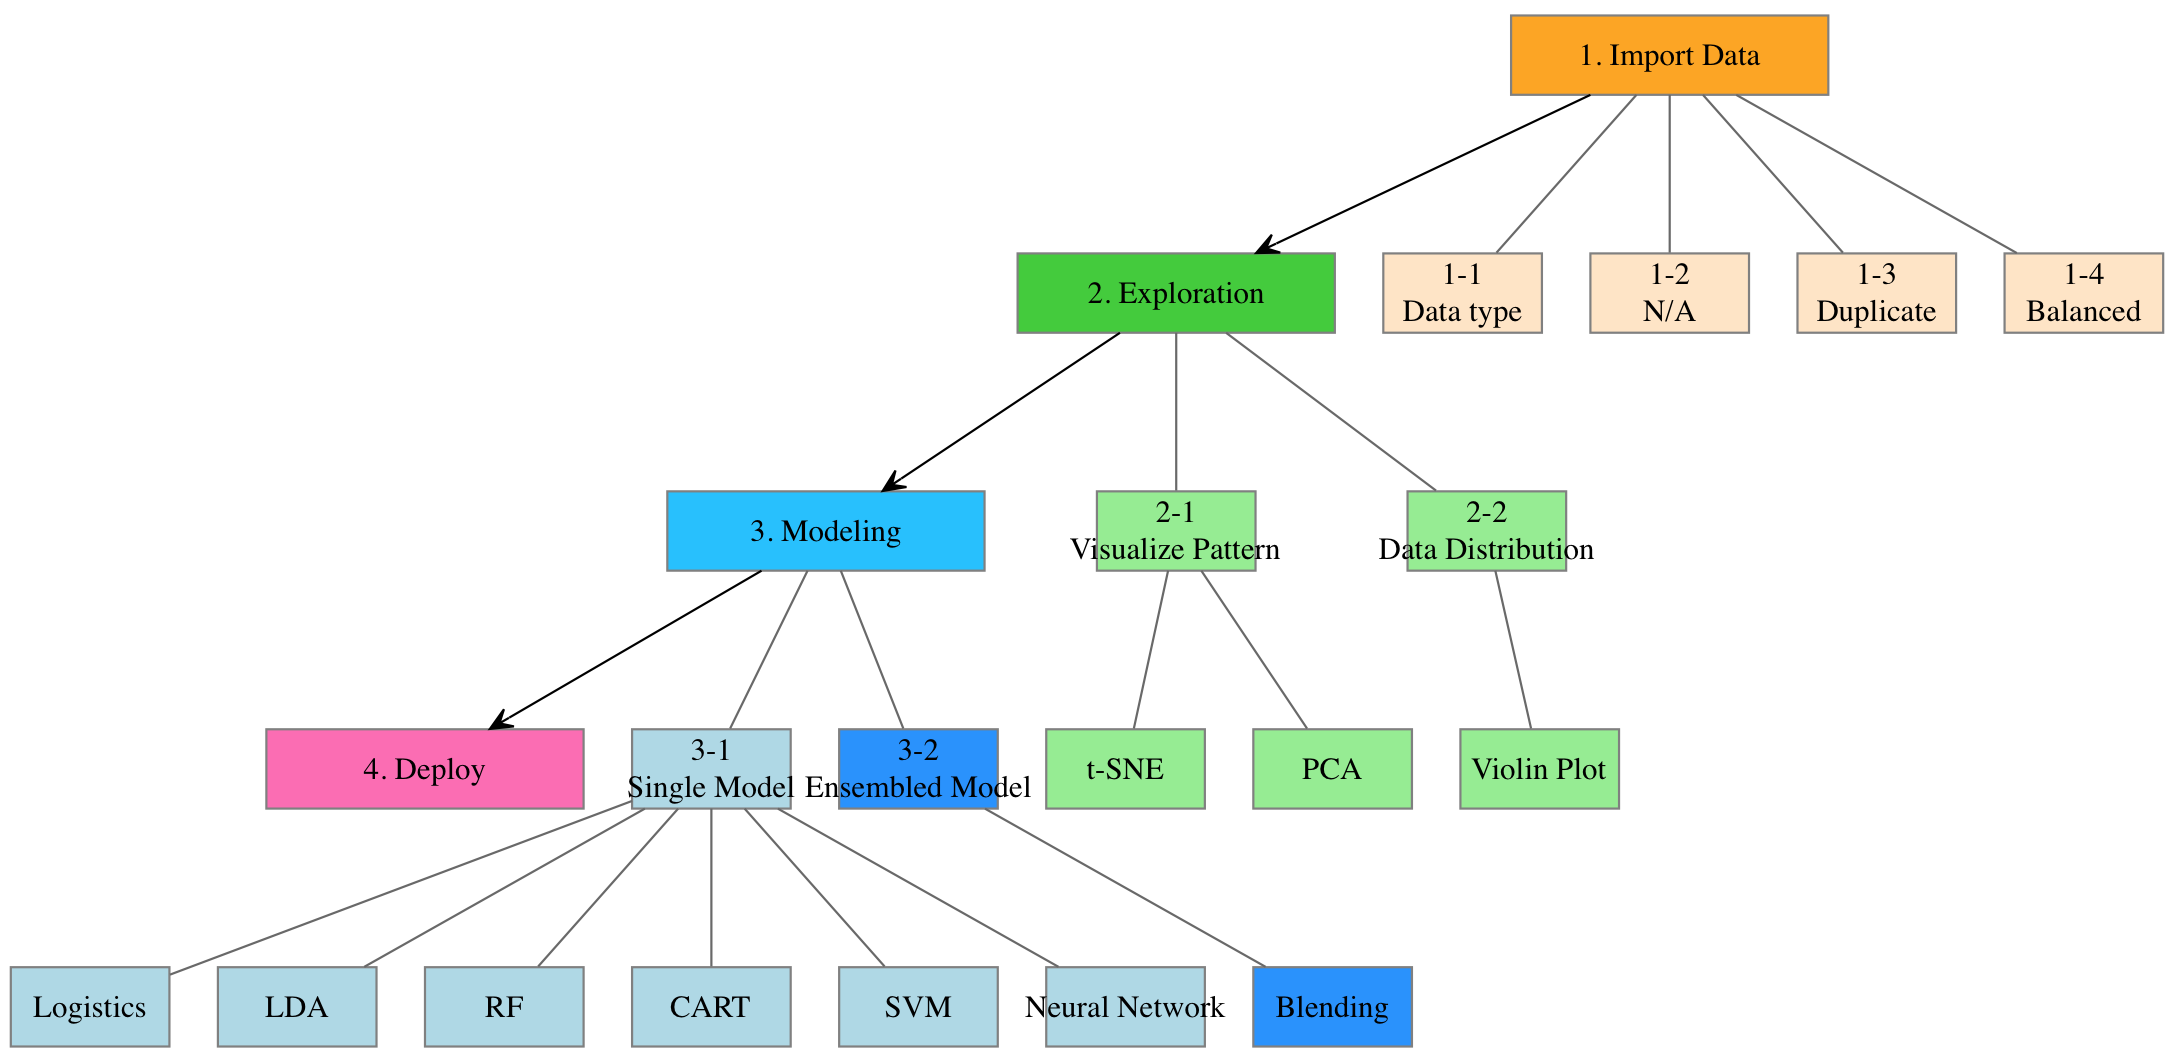
\includegraphics{pipeline}
	\caption{Workflow to solve the two-class classification problem. The workflow is mainly composed of four layers (with different color indicated).}
	\label{fig:1}
\end{figure*}
% Pipeline 

\section{Investigate dataset}

Keep in mind of various data type, e.g. categorical, numerical, etc. Only after having investigated the properties of dataset can I select suitable algorithms to deal with dataset of complexity. For example, linear regression requires numerical predictors and cannot accept nominal data. 

The following basics of our dataset are listed below: 
\begin{enumerate*}[label=(\roman*)]
	\item Feature No. 43 44 45 46 47 48 49  are binary indicators, i.e. 0/1,  while the rest are numbers (either integer or floating numbers).
	\item No N/A (missing value) exists. 
	\item Dataset contains duplicate entries. 
	\item Dataset is not balanced.
\end{enumerate*}
%	1)  2) 3)4) 

\subsection{Dataset contains duplicate samples}
Dataset (predictor matrix $X$ together with one column of labels $Y$) $D \in \mathbb{R}^{50000\times 78}$. The number of unique entries is 48948. Duplication will interfere with model training, thus the redundant are removed and the data matrix changes down to $\mathbb{R}^{48948\times 78}$. 

\subsection{Labels of samples are imbalanced}
\begin{marginfigure}
\centering
	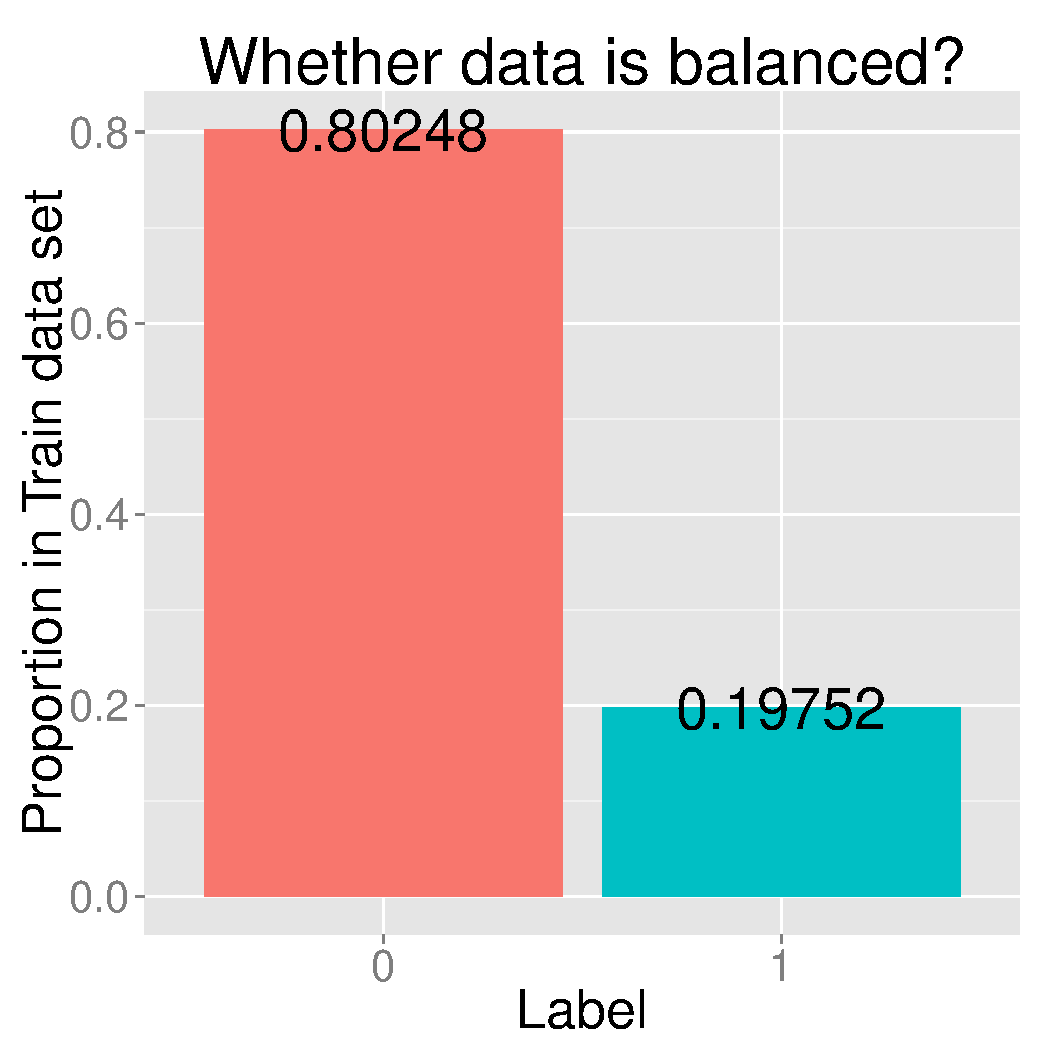
\includegraphics[width=0.5\linewidth]{data_balance}
	\caption{Barplot indicating the proportion of each label within the training dataset. The percentage of Label-0 and Label-1 is roughly 80\% and 20\% respectively.}
	\label{fig:dt-balance}
\end{marginfigure}

As shown in Figure-\ref{fig:dt-balance}, the labels (also called response) of training data are highly \textbf{imbalanced}. If modeling is using imbalanced data, classification models would be trained to be biased towards one category which is in particular true for algorithms like kMeans, kNN, therefore models would be more likely to fail on classifying unseen data. 

\subsection{Data is potentially separable}

Long before training classifier, I was wondering whether the data is separable. If intrinsic properties of data itself implied there is no way to be classified, more work on algorithms are hopeless. Therefore I would like to use \textbf{un-supervised models} to investigate and visualize the underlying pattern. 

\begin{marginfigure}
\centering
	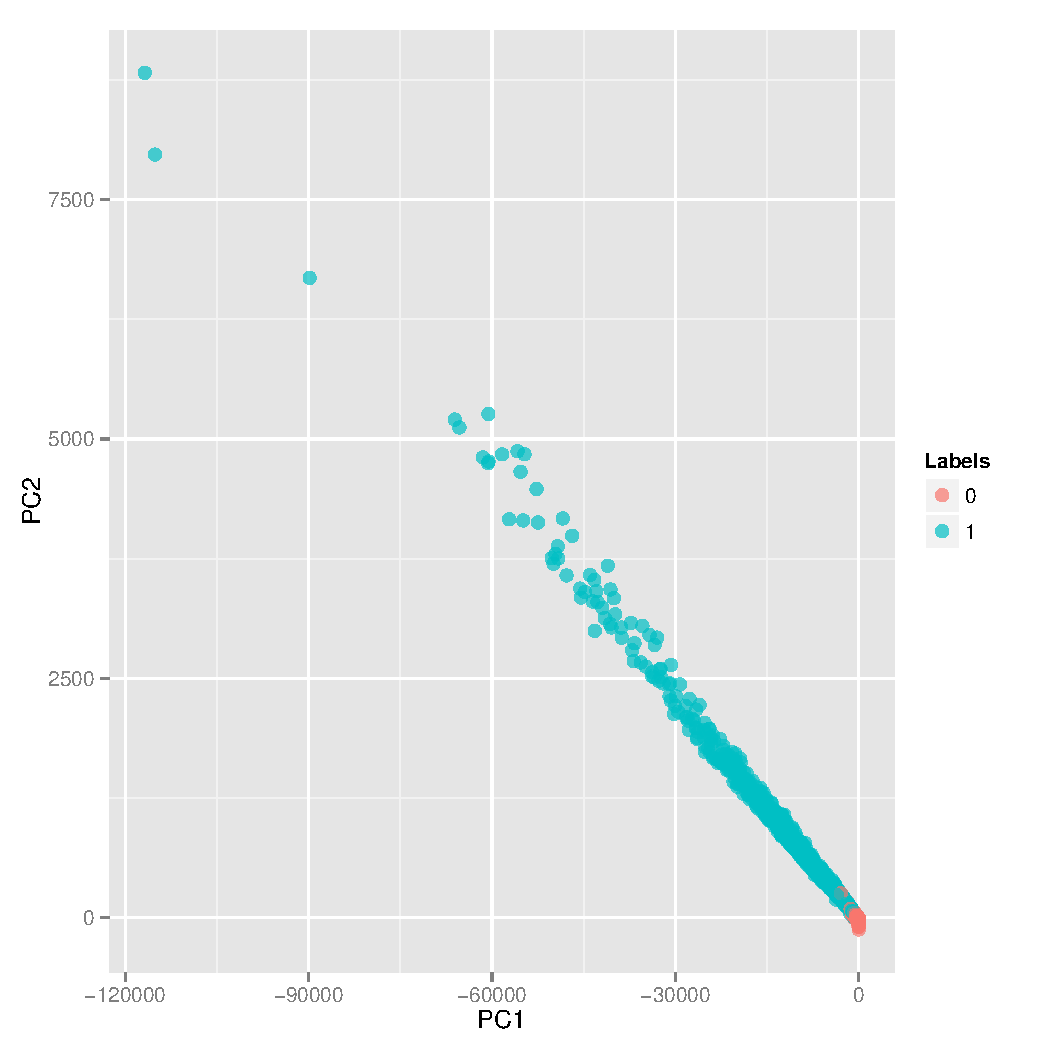
\includegraphics[width=0.5\linewidth]{pca_data_viz}
	\caption{Scatterplot showing the underlying structure of predictor matrix with ranking top-2 principle components as axises. Afterwards the color of each entry indicating its label is added. }
	\label{fig:pca_viz}
\end{marginfigure}

PCA was introduced during EigenFace class and considered as promising dimension reduction method, hence here PCA is applied on normalized predictor matrix $X$ and the first 2 PCs are extracted to visualize the entire predictor in 2-D scatter plot (See Figure-\ref{fig:pca_viz}). 

However, the PCA scatter plot could hardly reveal data pattern. This result is plausible because the first two PCs poorly explain variance thus much information are lost (See Figure-\ref{fig:pca_var}) and cannot be proper representatives of original full data. 

\begin{marginfigure}
\centering
	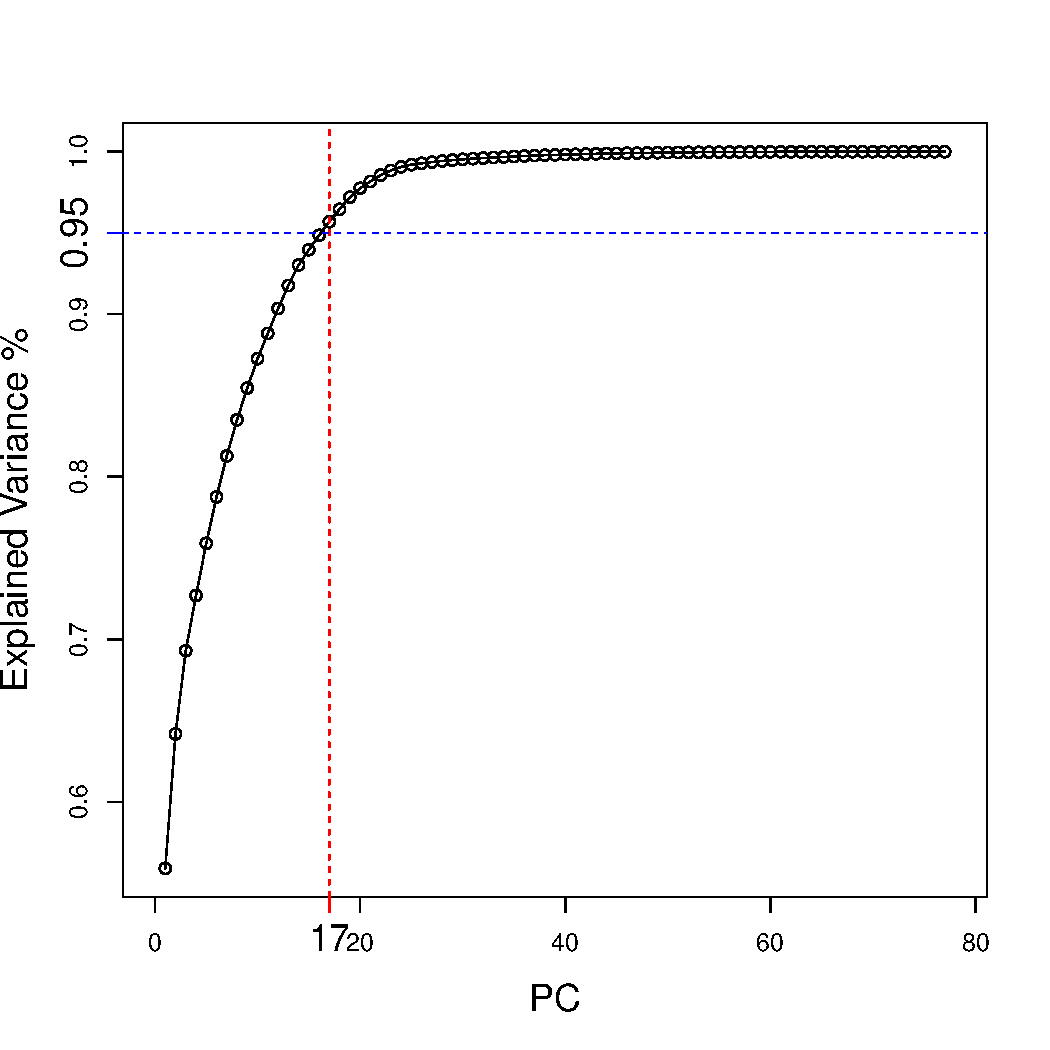
\includegraphics[width=0.9\linewidth]{pca_variance}
	\caption{Line plot showing the cumulatively explained variance over ordering principle components. Top 17 PCs (indicated by red dashed line) could explain at least 95\% variance (indicated by blue dashed line). Top 2 PCs can only explain 60-65\%.}
	\label{fig:pca_var}
\end{marginfigure}

I turn to t-SNE which is an un-supervised feature reduction approach and quite popular among Kaggle competition. 

%t-SNE requires input matrix being unique. 

Figure-\ref{fig:tsne} intuitively indicates the underlying structure of data is potentially separable within 2D space thus it gives me hope to figure out solutions for the two-class classification task on higher dimensional space.  

\begin{marginfigure}
\centering
	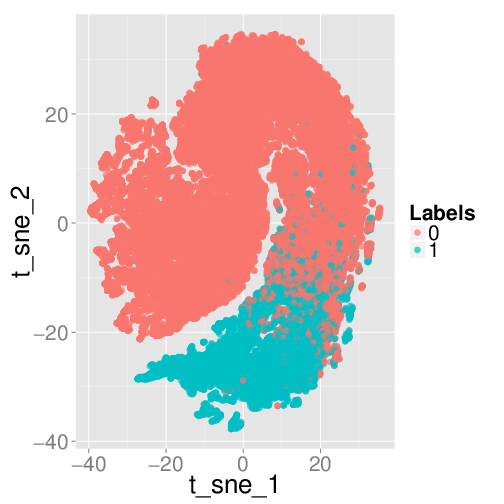
\includegraphics[width=0.5\linewidth]{tsne}
	\setfloatalignment{b}
	\caption{Scatterplot showing the result of t-SNE on unique predictor data matrix. Color indicating label of each entry is added afterwards. }
	\label{fig:tsne}
\end{marginfigure}

\section{Prepare training dataset and validating dataset}

\texttt{train.csv} (i.e. predictor matrix $X$) and \texttt{train\_label.csv} (i.e. response vector $Y$) together form our dataset $D$. Unique entries dataset $U$ is produced from raw dataset $D$ with duplication removed. 

As one of the strategies to avoid over-fitting, dataset $U$ will be randomly split into two subset dataset, i.e. training dataset $T$ and validating dataset $V$, which takes \textbf{80\% and 20\% }respectively. The dataset $T$ is for training model and dataset $V$ is for testing model performance. 

Therefore validating dataset $V$ here is actual test dataset. Because\texttt{test.csv} is supposed for evaluation instead of testing but it uses the name already, here comes word "validating" for dataset $V$ to maintain naming consistency. 

\section{Modeling and tuning}
Having tested logistic regression with different training settings (See \nameref{sec:append-a} Figure-\ref{fig:hilight-repcv}), I decide to perform \textbf{5-repeated 10-fold cross validation}. 

Furthermore to address data unbalance issue, subsampling method is used to recover balance of training dataset. For example, a classic method, down-sampling, will down-sample entries with Label-0 to same size as Label-1. But here a more complexed over-sampling approach is applied, which is called "\textbf{Random Over-Sampling Examples}" implemented in \texttt{ROSE} R language package (See \nameref{sec:method}). 

In sum, I decide to perform \textbf{subsampling during cross validation} to train models. %\cite{caretresubsmp}.

Because it is cross validation by which fashion the models are learning training dataset, ROC/AUC is available as metric for convergence condition. More importantly AUC is favored over accuracy, in particular our dataset is imbalanced. 

\subsection{Logistic Regression}
None

\subsection{LDA}
None

\subsection{CART}

\begin{marginfigure}[-8in] %manually set position
\centering
	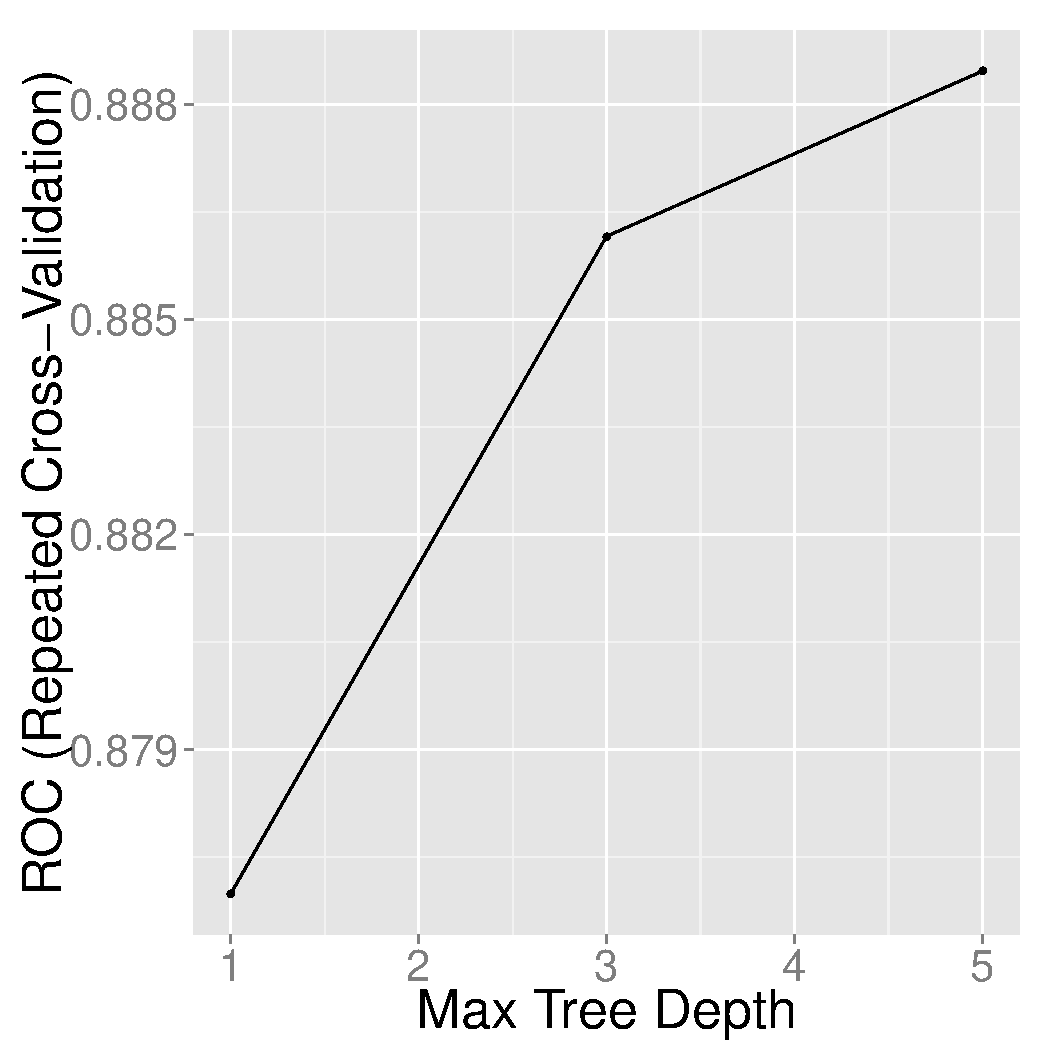
\includegraphics[width=0.6\linewidth]{cart_tuning}
	\caption{Tuning CART model with 3 settings}
	\label{fig:tune-cart}
\end{marginfigure}

\textit{Max Tree Depth}: Greater the depth, more-likely overfitting. See Figure-\ref{fig:tune-cart}. 

The trained tree structure is shown as Figure-\ref{fig:cart_tree}. 

\begin{marginfigure}[-4in]
\centering
	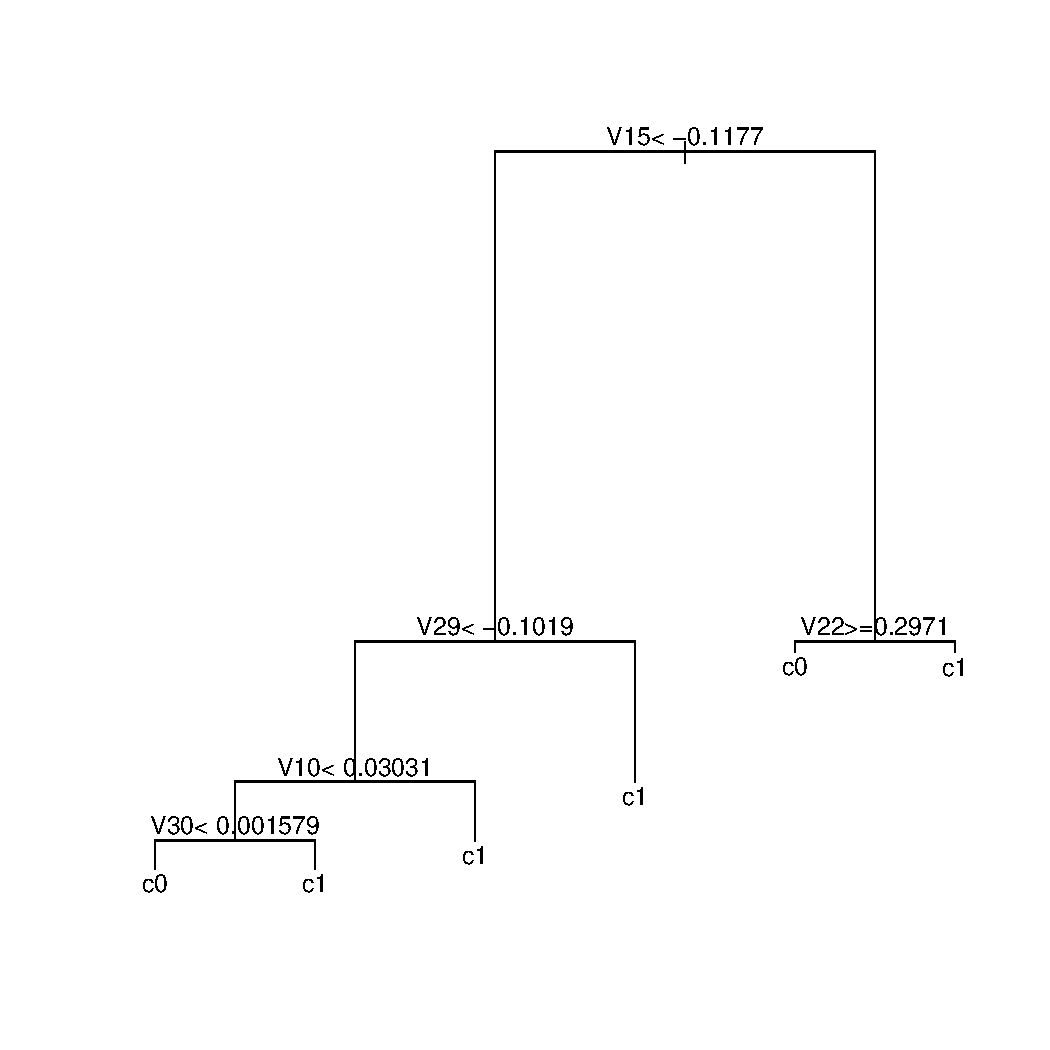
\includegraphics[width=0.9\linewidth]{cart_tree}
	\caption{Tree structure trained by CART algorithm. }
	\label{fig:cart_tree}
\end{marginfigure}

\subsection{Random Forest}

\textit{Number of randomly selected predictors}: Less predictors are selected, more-likely under-fitting. I tried three sets by selecting 5, 25, 55 predictors. See Figure-\ref{fig:tune-rf}.

\begin{marginfigure}
\centering
	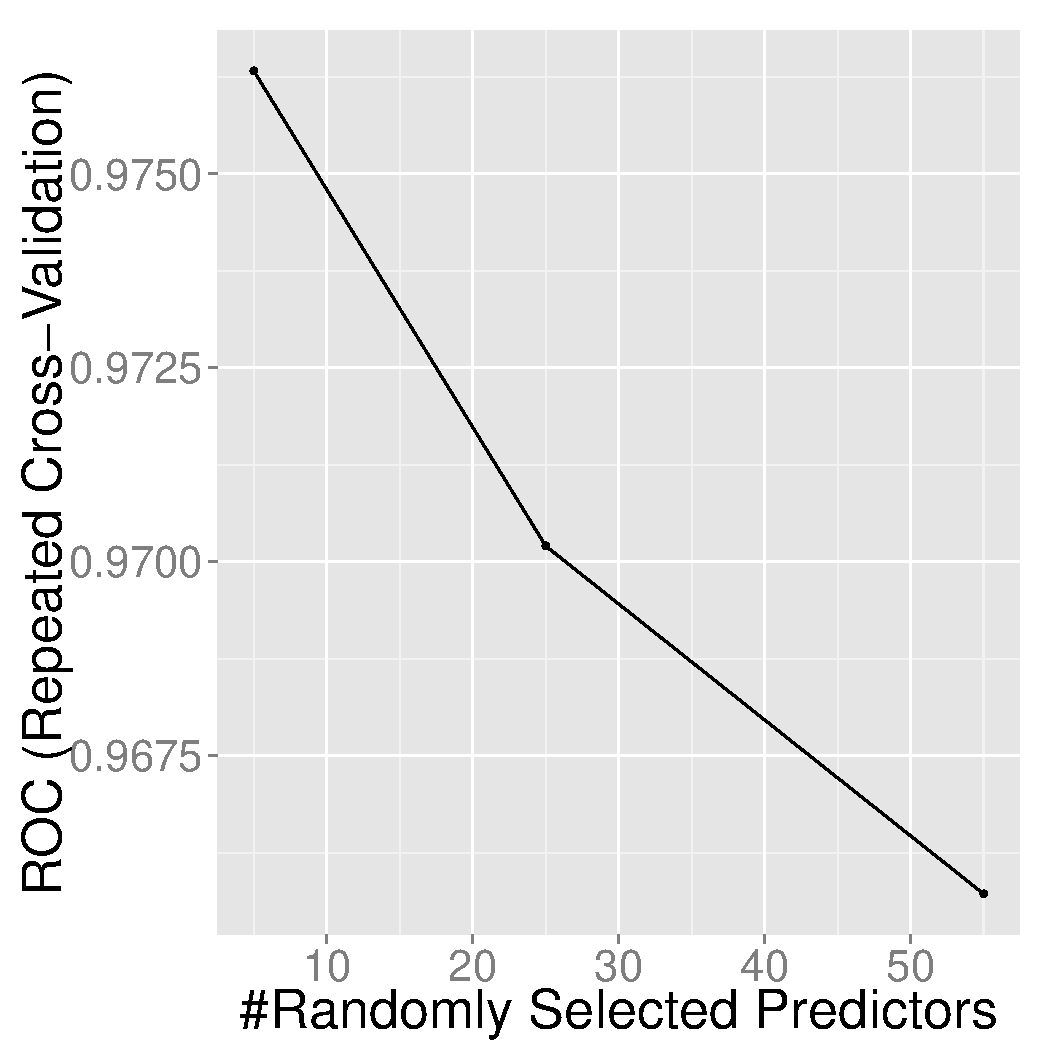
\includegraphics[width=0.6\linewidth]{rf_tuning}
	\caption{Tuning RF model with 3 settings}
	\label{fig:tune-rf}
\end{marginfigure}

\subsection{SVM (Linear)}
\textit{Cost}: Constant of the regularization term in the Lagrange formulation to control the soft margin. I set it as constant $C = 1$ thus no tuning for linear SVM. 

%\subsection{SVM (Radial)}
%1) \textit{Cost}: ditto; 2) \textit{Sigma}: denominator of the radial basis function kernel. See Figure-\ref{fig:tune-svm-rad}.
%
%\begin{marginfigure}
%\centering
%	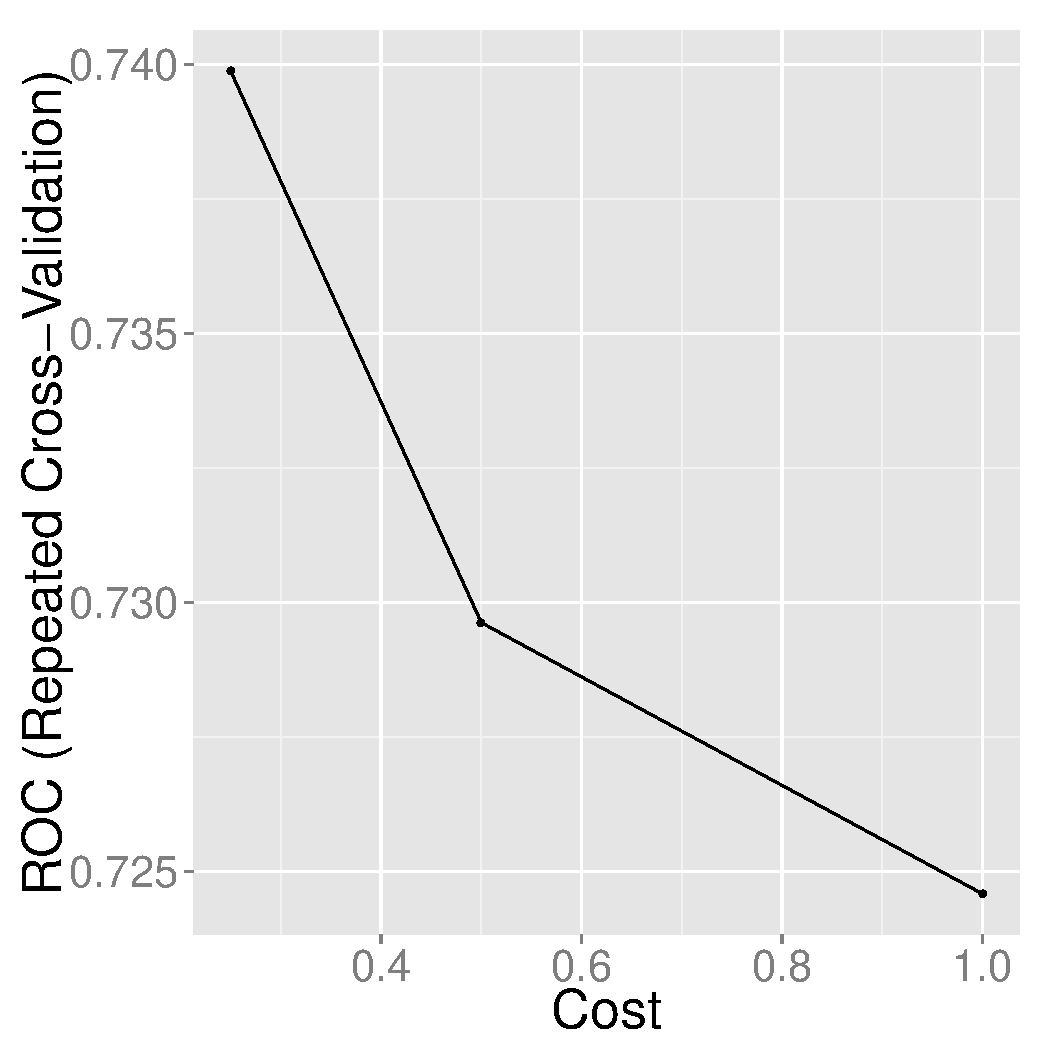
\includegraphics[width=0.6\linewidth]{svm_radial_tuning}
%	\caption{Tuning SVM with radial basis kernel function with 3 settings}
%	\label{fig:tune-svm-rad}
%\end{marginfigure}

\subsection{Neural Network}
1) \textit{Number of hidden units}: more hidden units, more-likely overfitting; 2) \textit{Weight decay}: controls the training process.

See Figure-\ref{fig:tune-nn}. 
\begin{marginfigure}
\centering
	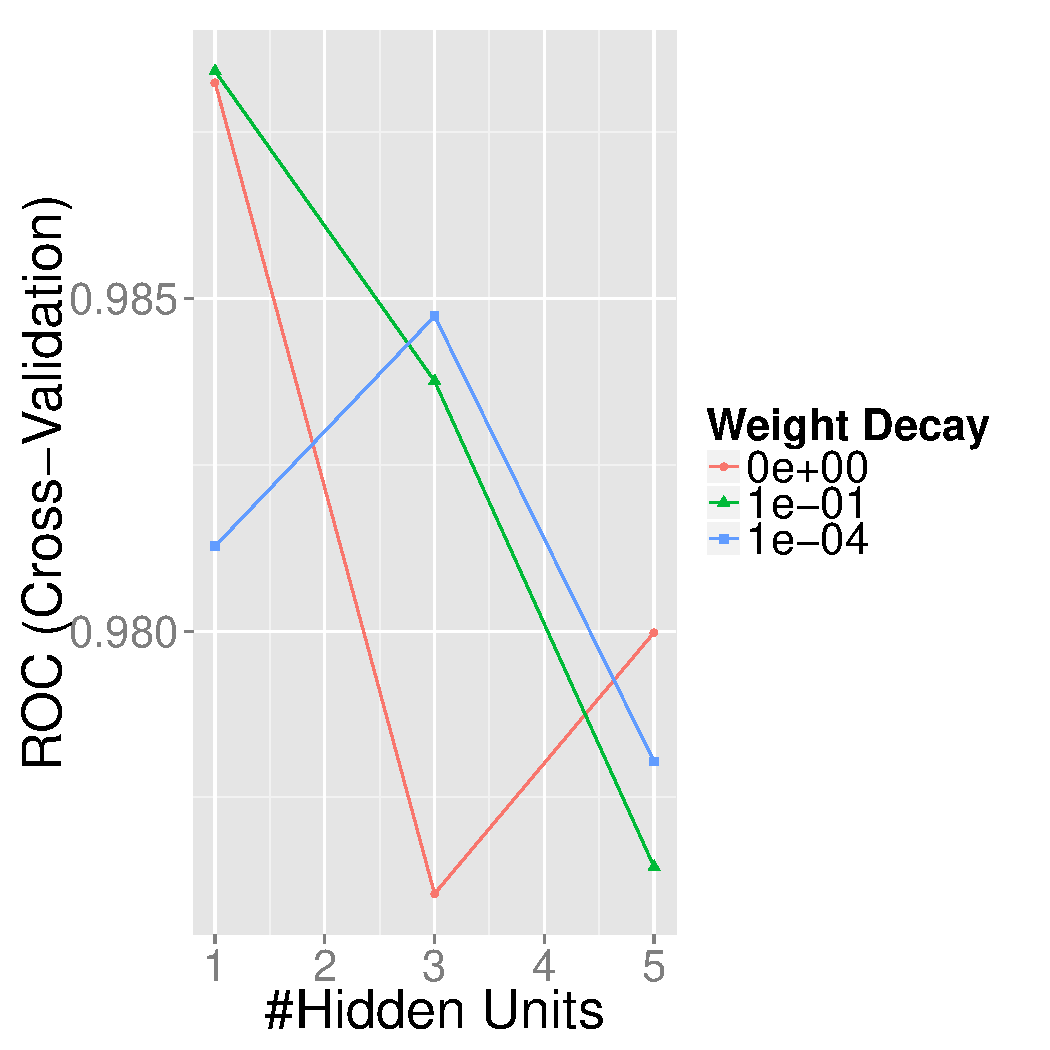
\includegraphics[width=0.6\linewidth]{nn_tuning}
	\caption{Tuning neural network with 3 settings }
	\label{fig:tune-nn}
\end{marginfigure}

\subsection{Ensemble Model}

Having trained all the above 7 models, I turn to an advanced topic : ensemble model which combines the power of wisdom of group \cite[0.5cm]{mlwave}. Specifically \textbf{blending} method fits my need. 

I set up a "voting committee" with all the 7 trained models as members to determine the label of unseen data. The committee is implemented by logistic regression model for convenience, and each model trained previously is one feature of the model. 

In details, each model will report the probability of unseen sample being "Label-0", rather than categorical label. The results of individual models will be feature spaces of ensemble model which is a new logistic regression model. The work for constructing the blending model is equivalent to building a logistic regression with numerical inputs and binary labels as output. 

%\break
\section{Performance and Blending model is best}

Performance of all 7 models is shown as Figure-\ref{fig:perf_singles}. Logistic regression and SVM (Linear kernel) are top best individual models.   

\begin{marginfigure}[-1in]
\centering
	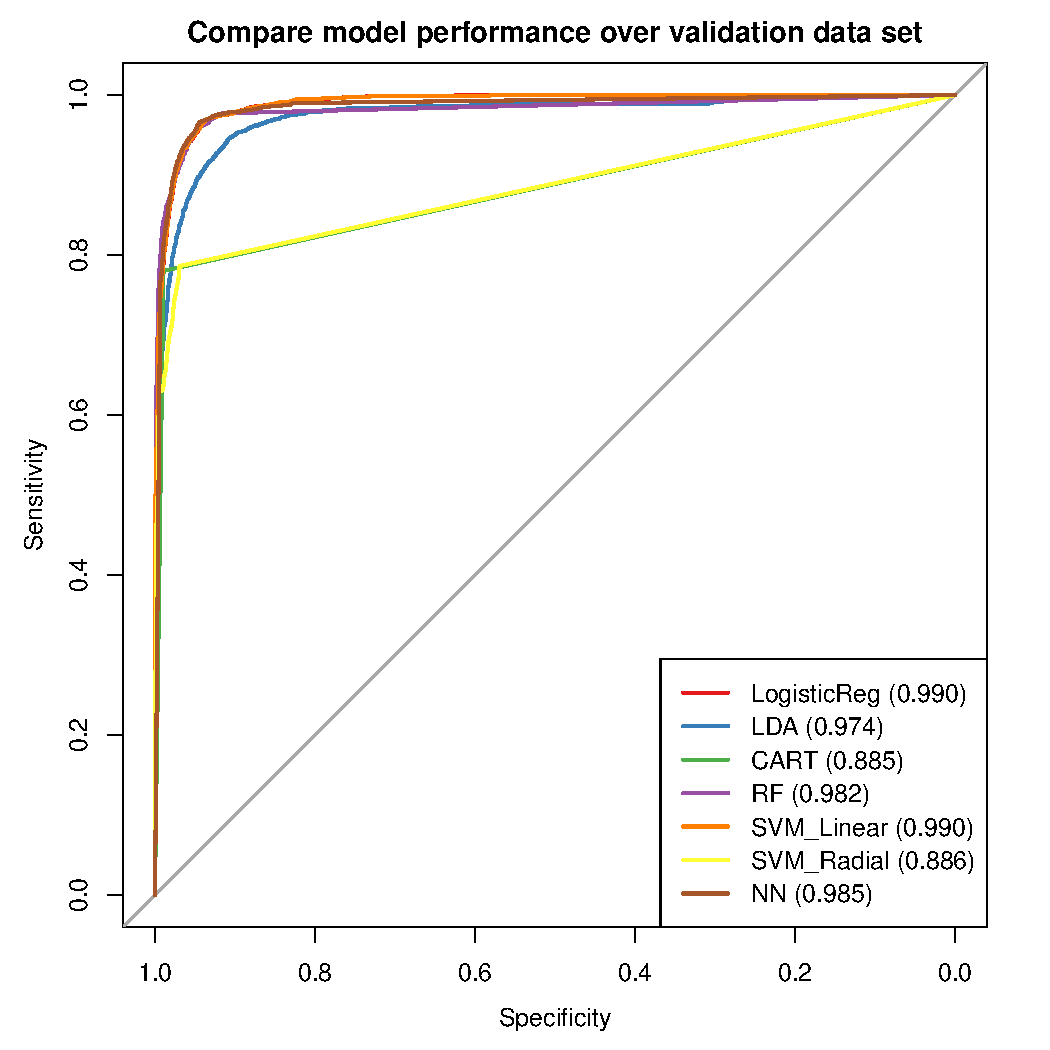
\includegraphics[width=0.8\linewidth]{compare_single_models}
	\caption{Performance of 7 models, i.e. logistics regression, LDA, RF, CART, SVM(linear), SVM(radial), Neural Network. ROC/AUC is estimated by applying models on independent validating dataset and AUC values are attached to model names on bottom right. }
	\label{fig:perf_singles}
\end{marginfigure}

Shown as Figure-\ref{fig:perf_blend}, blending model (AUC = 0.990) is superior to any other individual model, except logistic regression and SVM. Blending model is neither dominated by nor exactly same as individual models (results not shown here), therefore having same AUC values does not imply they are same model, but rather means they have same performance and prediction ability

Furthermore, the unseen test (evaluation) dataset is expected to be complexed, therefore it is better to deploy blending model which take multiple factors into account. 

\begin{marginfigure}
	\centering
	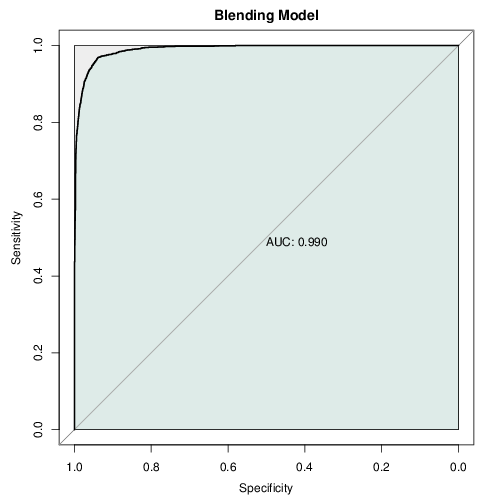
\includegraphics[width=0.8\linewidth]{blending_perfm}
	\setfloatalignment{b}
	\caption{Performance of blending model. ROC/AUC is estimated by applying model on independent validating dataset. Blending model achieves AUC $=0.990$, which is superior to any other individual model. }
	\label{fig:perf_blend}
\end{marginfigure}

\section{Deploy}

Read-in the \texttt{test.csv} and feed its predictor matrix to my blending model, so that labels are generated as final results. 

\break
\section{Methods}\label{sec:method}

Entire workflow is implemented by using R language with standard packages, in particular \texttt{caret}\cite{maxcaret} (short for Classification And REgression Training). It attempts to provides uniform syntax to call other existed R packages to build machine learning workflow. 

Compared with Matlab requiring commercial licenses, R is a free software environment for statistical computing and graphics. More important, it can natively employ C/C++ codes to implement packages to avoid running slow, while Matlab is mostly slow. As our data is relatively big and advanced algorithm are involved, e.g. SVM, random forest, neural network, it is wise to select a language with both professional statistics and machine learning ability and also running efficiency. 

Entire work was designed and implemented independently by Yun Yan. 

\subsection{t-SNE: unique predictor v.s. unique sample} 
Unique predictor matrix and unique samples are two different concepts because sample = predictor vector + label scalar. Two samples might share the same predictor vector but differ at binary label. It is important to investigate these possible events, because in this case model learning  becomes much more challenging. In addition, only with extra data pre-processing, can t-SNE \cite{tsne,van2008visualizing} be used to intuitively check whether dataset is separable. As unsupervised learning technique, t-SNE accepts predictor matrix alone. It is afterwards when label information is added into 2D scatterplot. There is labeling collision for two samples with same predictor vector but distinct labels. 

Good news is that these cases do not exist in our dataset, which allows me to directly apply t-SNE for data visualization. 

\subsection{Model training packages}

\begin{table}[hb]
\centering
\begin{tabular}{lll}
\toprule
\textbf{Model} & \textbf{Method of \texttt{caret}} & \textbf{R package} \\
\midrule
Logistic Regression & \texttt{glm} & stats\\
LDA &  \texttt{lda} & MASS\\ 
CART &  \texttt{rpart2} & rpart\\
Random Forest & \texttt{rf} & randomForest\\
SVM (Linear) & \texttt{svmLin} & kernlab\\
%SVM (Radial) & \texttt{svmRadial} & kernlab\\
Neural Network & \texttt{nnet} & nnet\\
\bottomrule
\end{tabular}
%\setfloatalignment{b}
\caption{List of dependencies for implementation. Second column gives the \texttt{method} name required by \texttt{caret} package to perform selected algorithm.}
\label{tab:model-packages}
\end{table}

\subsection{General usage of \texttt{caret}}
First is the general settings to perform subsampling (ROSE) during 5-times repeated 10-fold cross validation. 

\begin{lstlisting}[language=R]
trCtrolRepCV <- trainControl(method = 'repeatedcv', number = 10, 
                             repeats = 5, 
                             sampling = 'rose', 
                             classProbs = TRUE, 
                             summaryFunction = twoClassSummary)
\end{lstlisting}

Then we take LDA as example. It is by calling function named \texttt{train} to run model learning. Before actual modeling,  \texttt{train} function will normalize dataset as required by user. Finally "ROC" is used as \texttt{metric}. 

\begin{lstlisting}[language=R]                             
mdl_lda <- train(Label ~ . ,       # Formula: Label ~ Response matrix
                 data = train_df, # Dataset D = [X | Y]
                 method = "lda",  
                 trControl = trCtrolRepCV, 
                 preProcess = c('center', 'scale'), 
                 metric = "ROC")
\end{lstlisting}

The other individual models share the similar syntax. 

\subsection{Platform and software versions}

\noindent Ubuntu 14.04.3 LTS (GNU/Linux 3.13.0-68-generic x86\_64)

Intel(R) Xeon(R) CPU E5-2630L v2 @ 2.40GHz

R version 3.2.2 (2015-08-14)

%\break
\section{Appendix-A}\label{sec:append-a}
In order to determine general training strategy, logistic regression model is trained to learn demo training dataset (random 1500 samples). 
%\subsection{Data range of features implies need of normalization}
%
%Data range of features in the dataset varies a lot (figure not shown here). It indicates the necessary to normalize data. 

% supplement figures
\subsection{Highlight usage of repeated CV}
\begin{marginfigure}[-7in]
	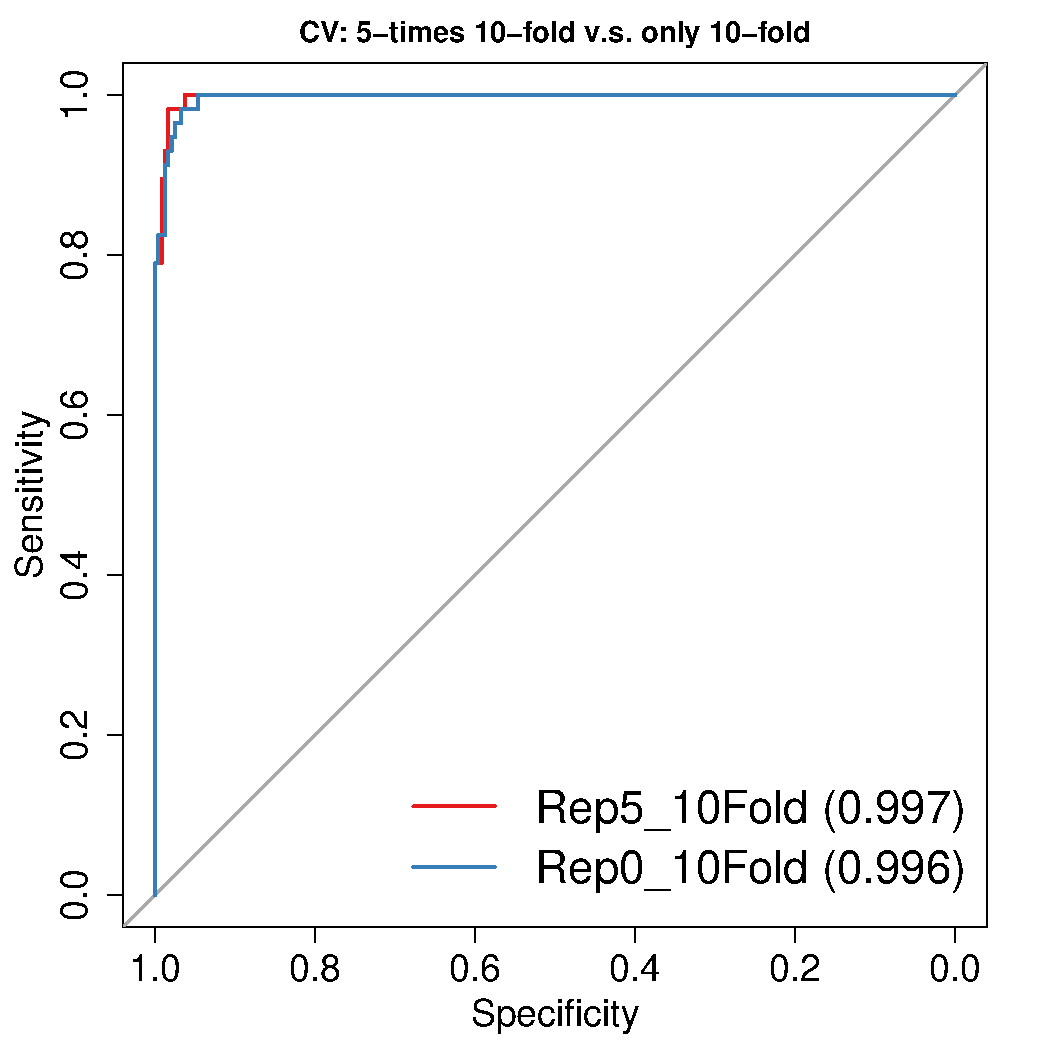
\includegraphics[width=0.9\linewidth]{hilit_repCV}
	\caption{ROC curve for logistic regression model with different training settings: 10-fold CV alone v.s. 5-repeated 10-fold CV. AUC is calculated by applying model on independent validating dataset. }
	\label{fig:hilight-repcv}
\end{marginfigure}
Using logistic regression as basic model, I tested performance with different CV settings: repeated CV v.s. CV alone (See Figure-\ref{fig:hilight-repcv}). Hence 5-times repeated 10-fold CV is superior to 10-fold CV alone, admittedly AUC did not improve much. 
 
\subsection{Highlight usage of subsampling}
\begin{marginfigure}[-2in]
	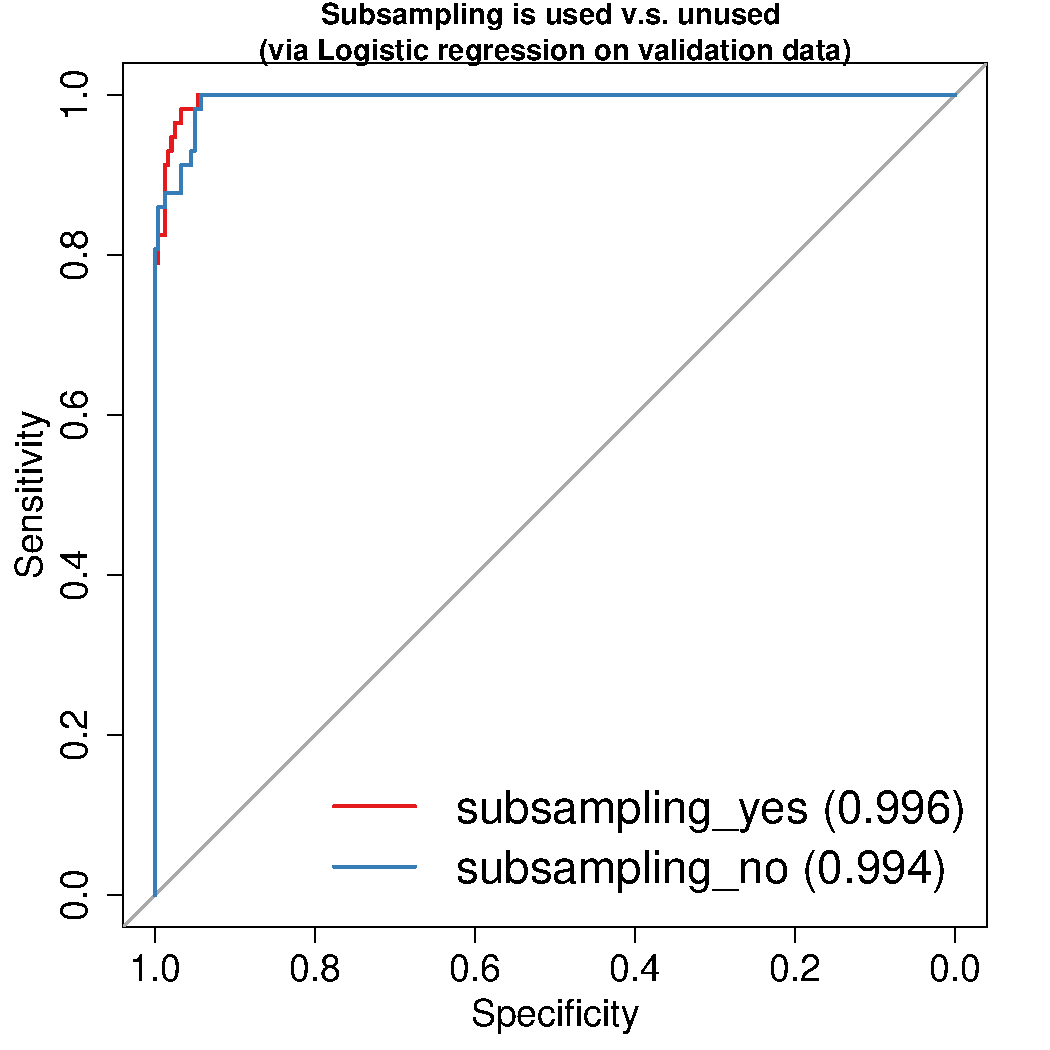
\includegraphics[width=0.9\linewidth]{hilit_subsampling}
	\caption{ROC curve for logistic regression model with different training settings: Subsampling during CV v.s. Without subsampling. AUC is calculated by applying model on independent validating dataset. }
	\label{fig:hilight-subsamp}
\end{marginfigure}
To deal with imbalanced training dataset, I investigated whether subsampling during resampling improves model performance. The answer is yes, as expected (See Figure-\ref{fig:hilight-subsamp}). 

%\break
\section{Appendix-B: Matlab}\label{sec:append-b}
% Matlab processing

This appendix shows how I train 4 models with KNN (with/without PCA), Linear Discriminant, SVM algorithms by using \textbf{Matlab} alone, specifically Statistics and Machine Learning Toolbox which has friendly GUI. 

Firstly, when importing data via graphic interface (See Figure-\ref{fig:matlab-import}). \texttt{train.csv} and \texttt{train\_label.csv} are merged before being imported. Specify the last column (i.e. label) of merged dataset as "response" in the GUI.

\begin{marginfigure}
	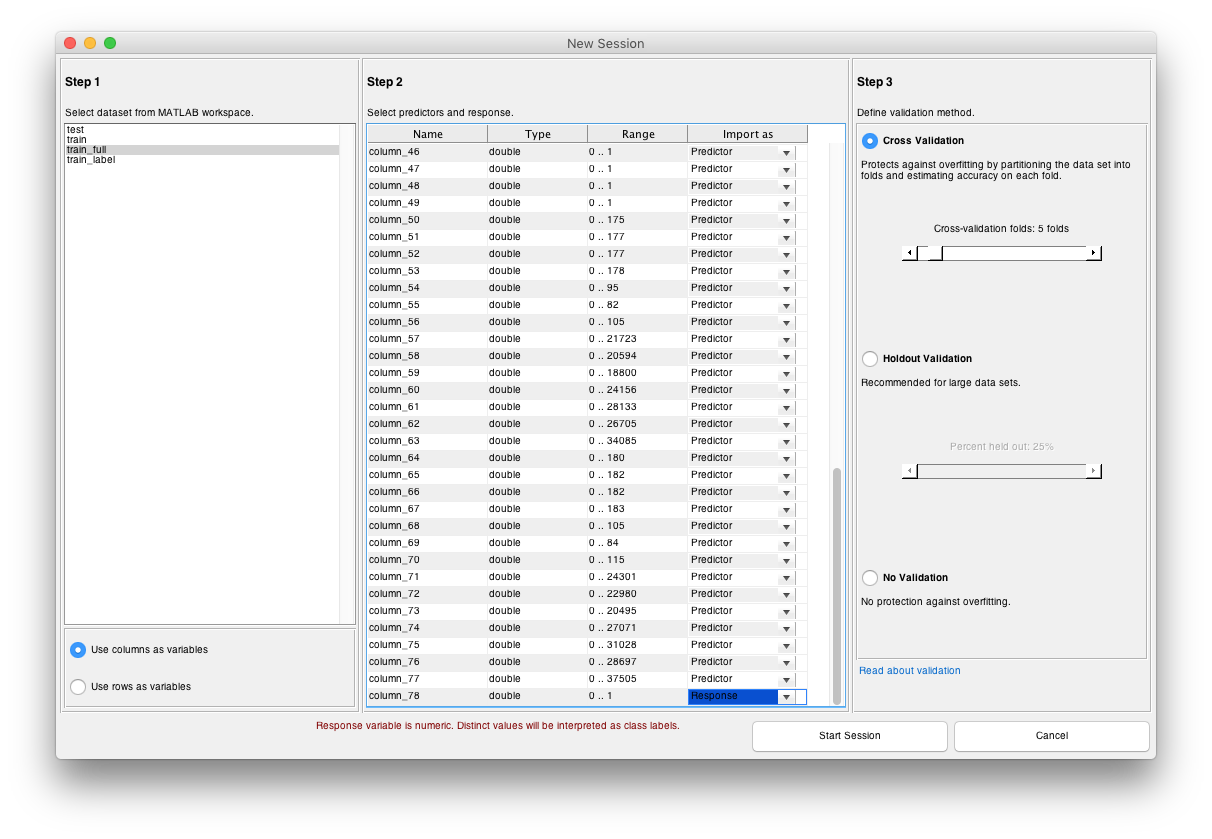
\includegraphics{matlab_step1_import}
	\caption{Importing data from Matlab workspace with statistic and machine learning toolbox. }
	\label{fig:matlab-import}
\end{marginfigure}

Secondly, train models. On top-left "Data browser" window, I have already trained 4 models, marked with accuracy on train dataset. The first one is KNN with cosine similarity as distance metric (See Figure-\ref{fig:knn-1}). It turns on PCA option to do dimension reduction. The detailed specs are available on bottom-left window. On right panel, its performance over training dataset is available, e.g. its AUC is 0.97. Noticed that these information about ROC curve can NOT be used to evaluate model performance because AUC is estimated over training set, rather than test test. 

Third, it is straightforward to train other models with click-run operations thanks to GUI. See the results as shown in Figure-\ref{fig:knn-1}, \ref{fig:knn-2}, \ref{fig:lda}, \ref{fig:svm}. 

\begin{figure*}[ht]
	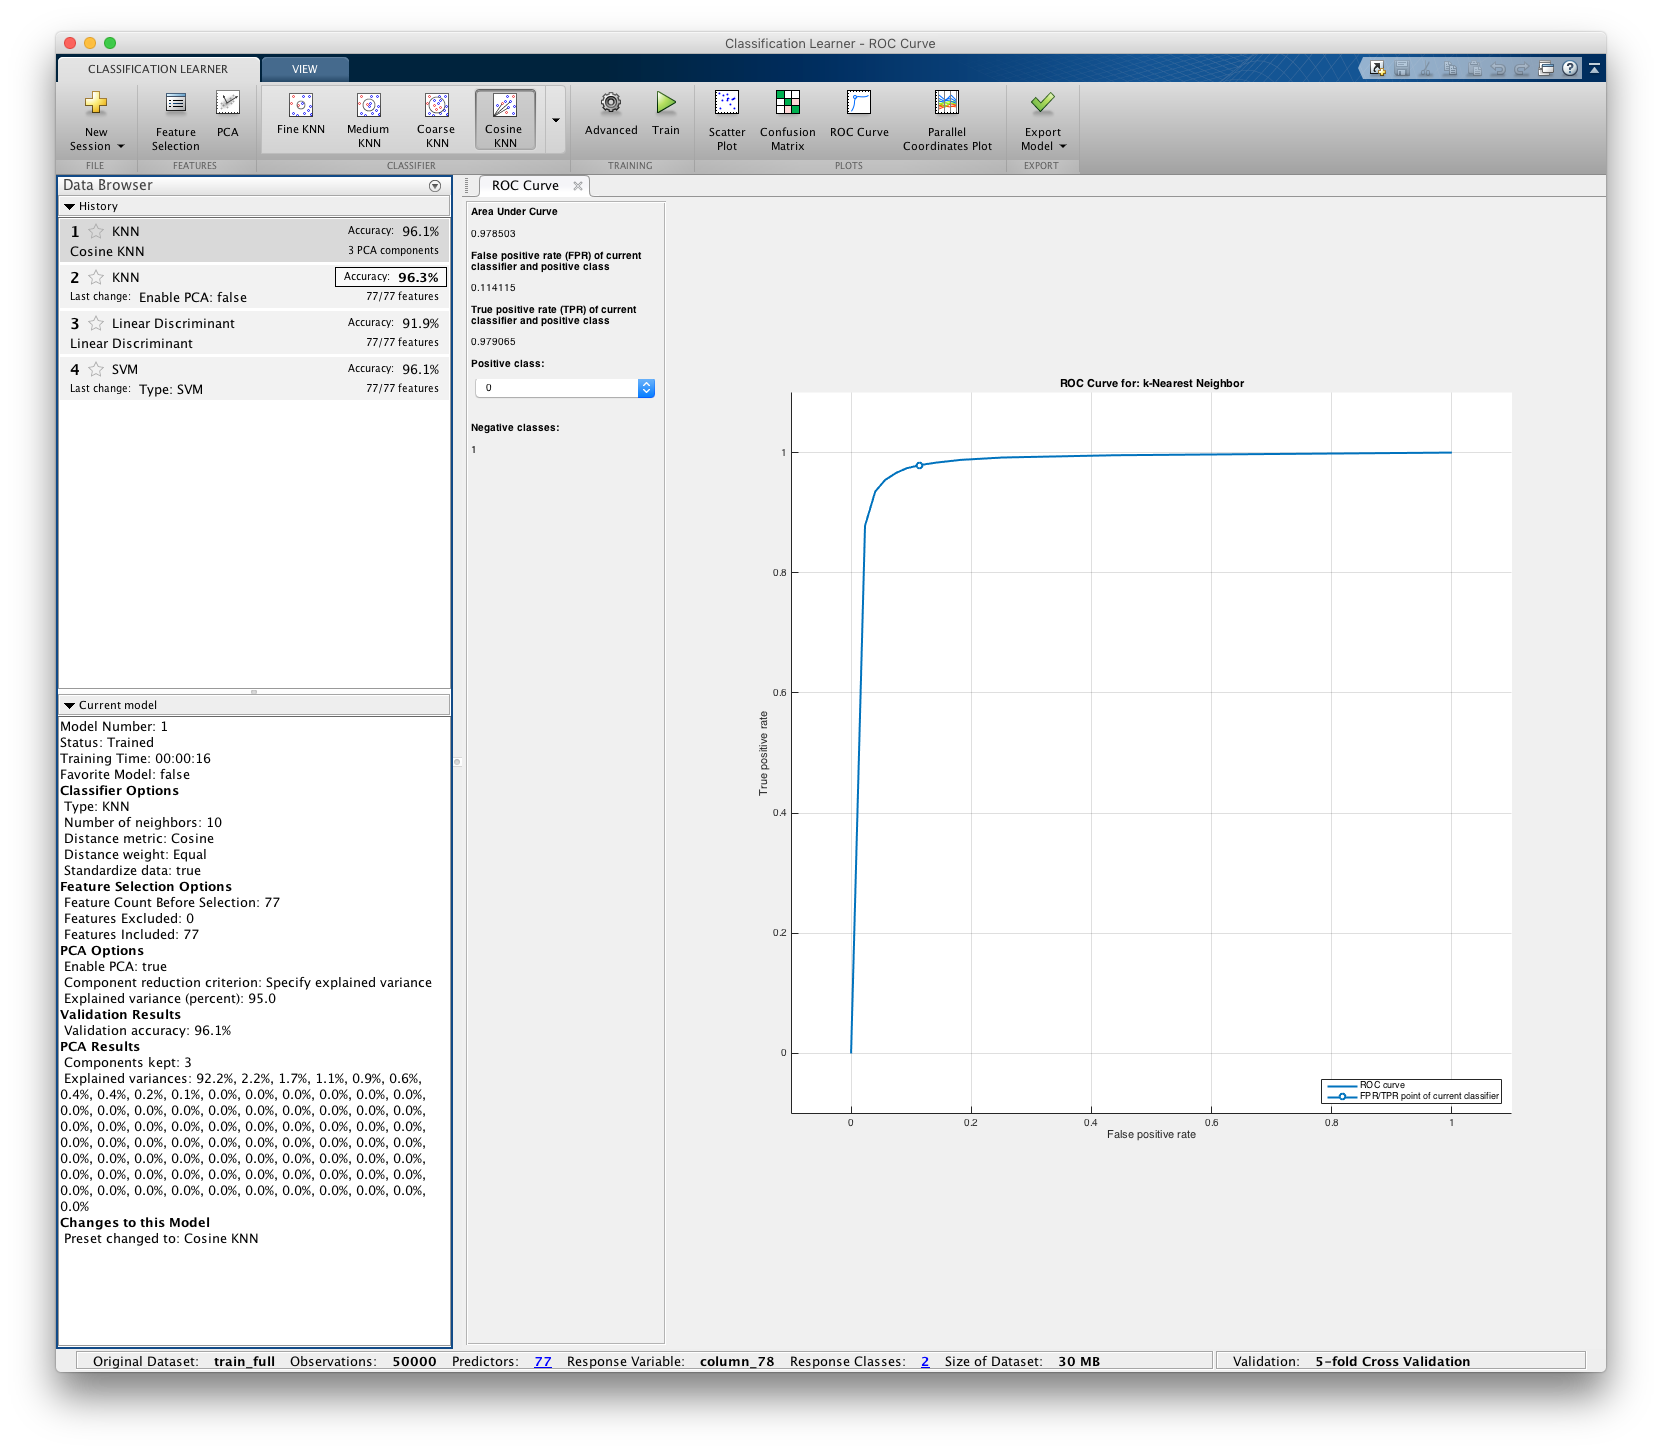
\includegraphics{matlab_train_m1}
	\caption{First KNN model details. Distance metric: cosine similarity; PCA: enabled. }
	\label{fig:knn-1}
\end{figure*}

\begin{figure*}[ht]
	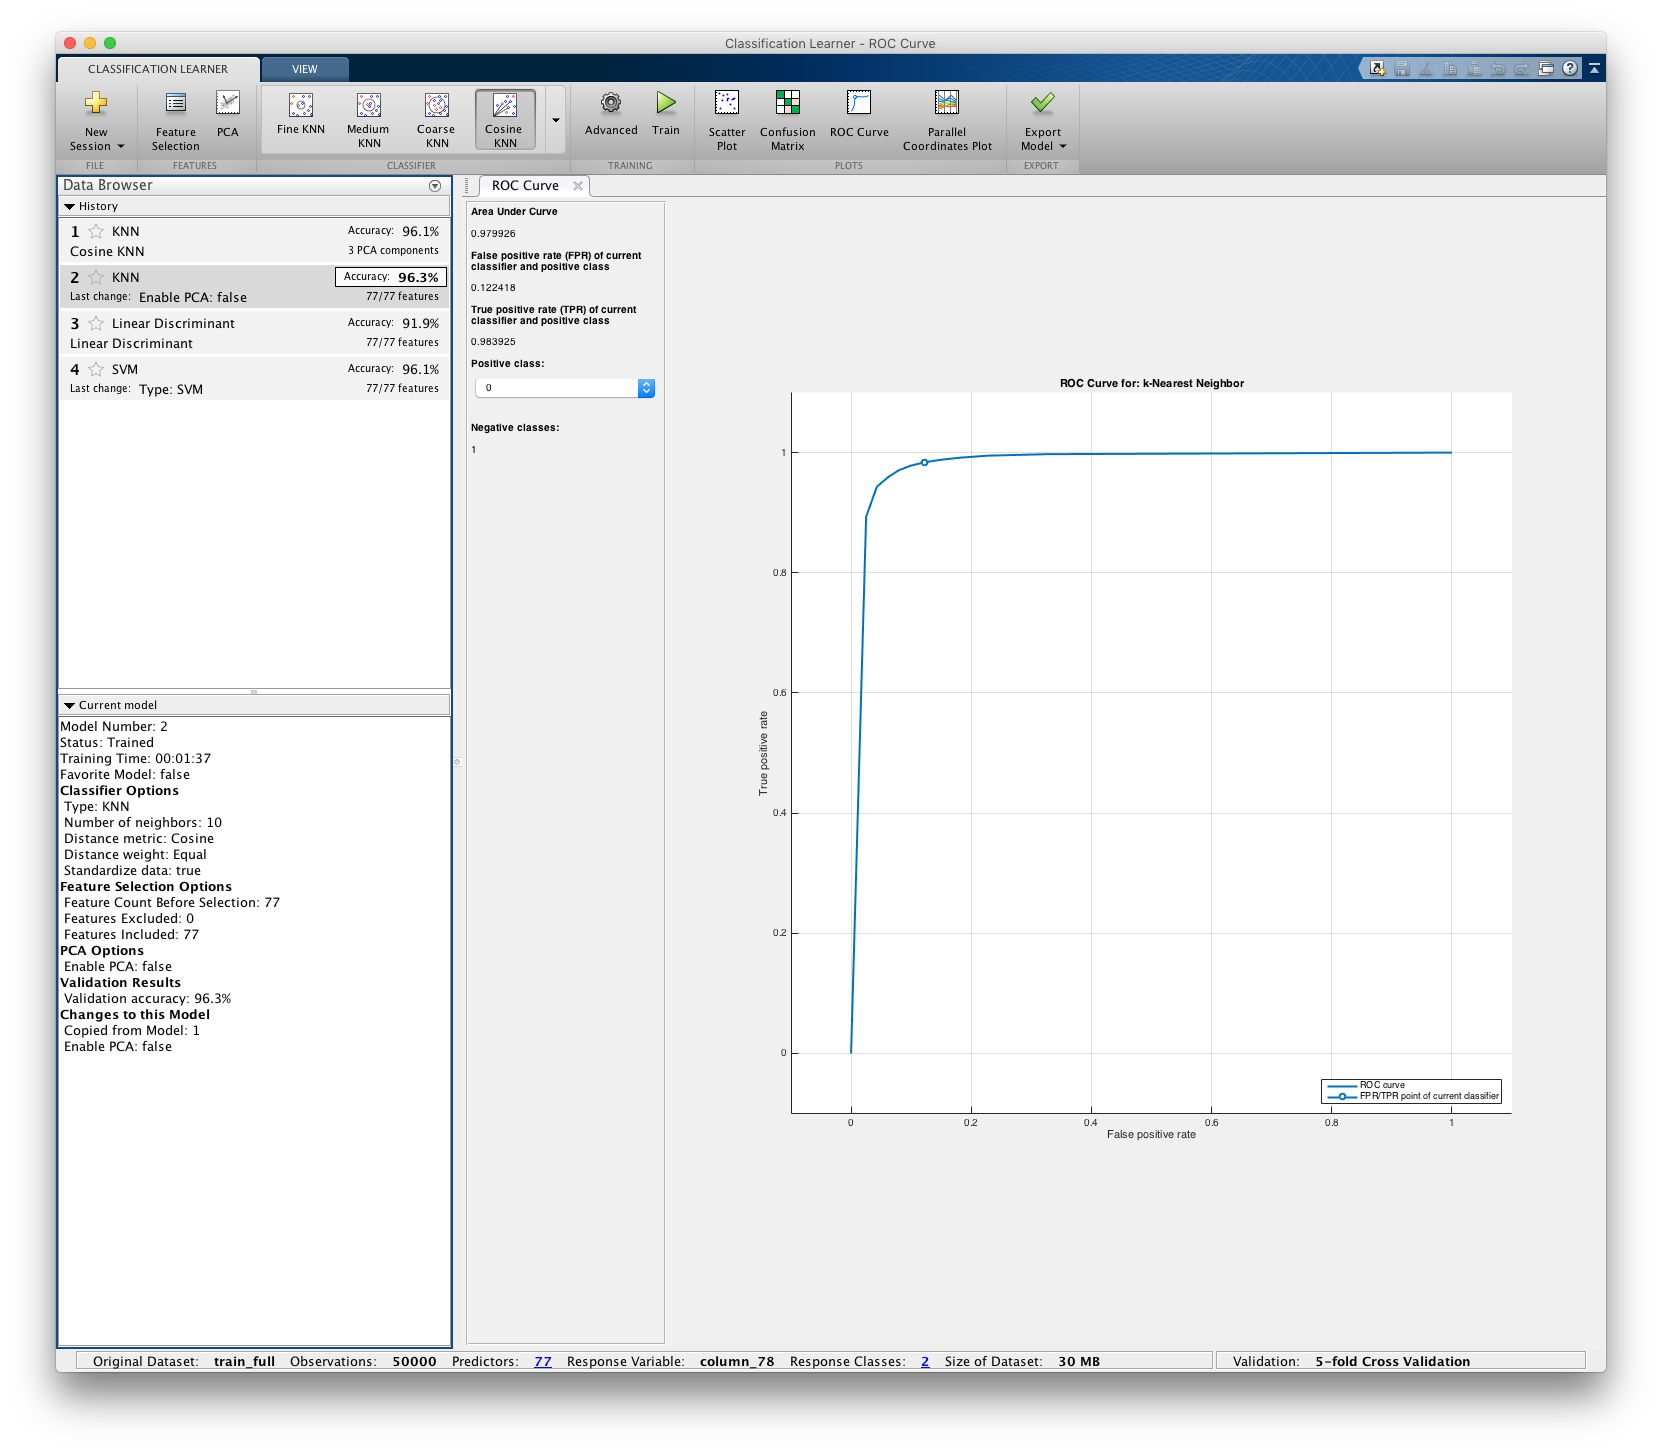
\includegraphics{matlab_train_m2}
	\caption{Second KNN model details.Distance metric: cosine similarity; PCA: disabled. }
	\label{fig:knn-2}
\end{figure*}

\begin{figure*}[ht]
	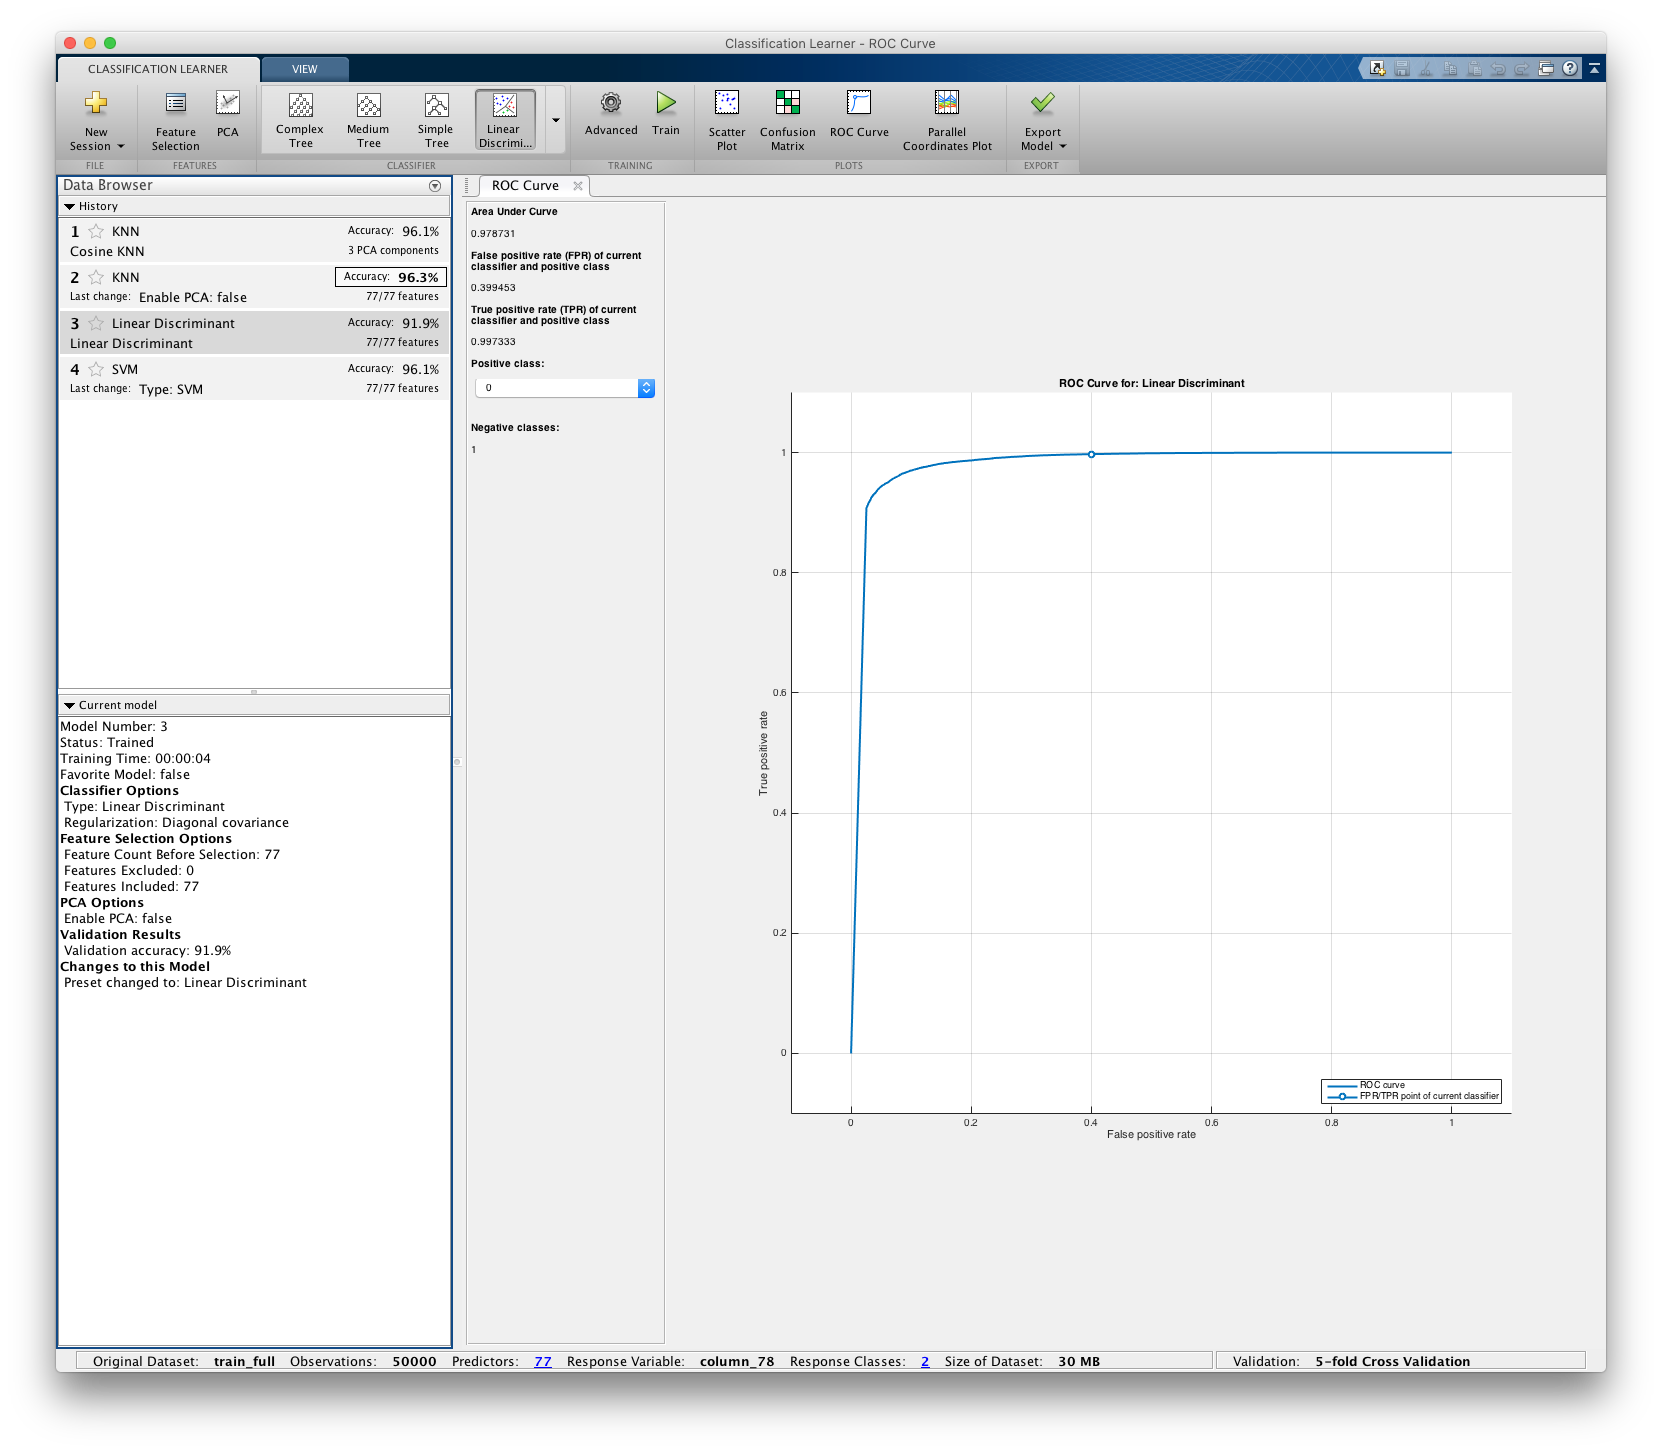
\includegraphics{matlab_train_m3}
	\caption{Third model: LDA. }
	\label{fig:lda}
\end{figure*}

\begin{figure*}[ht]
	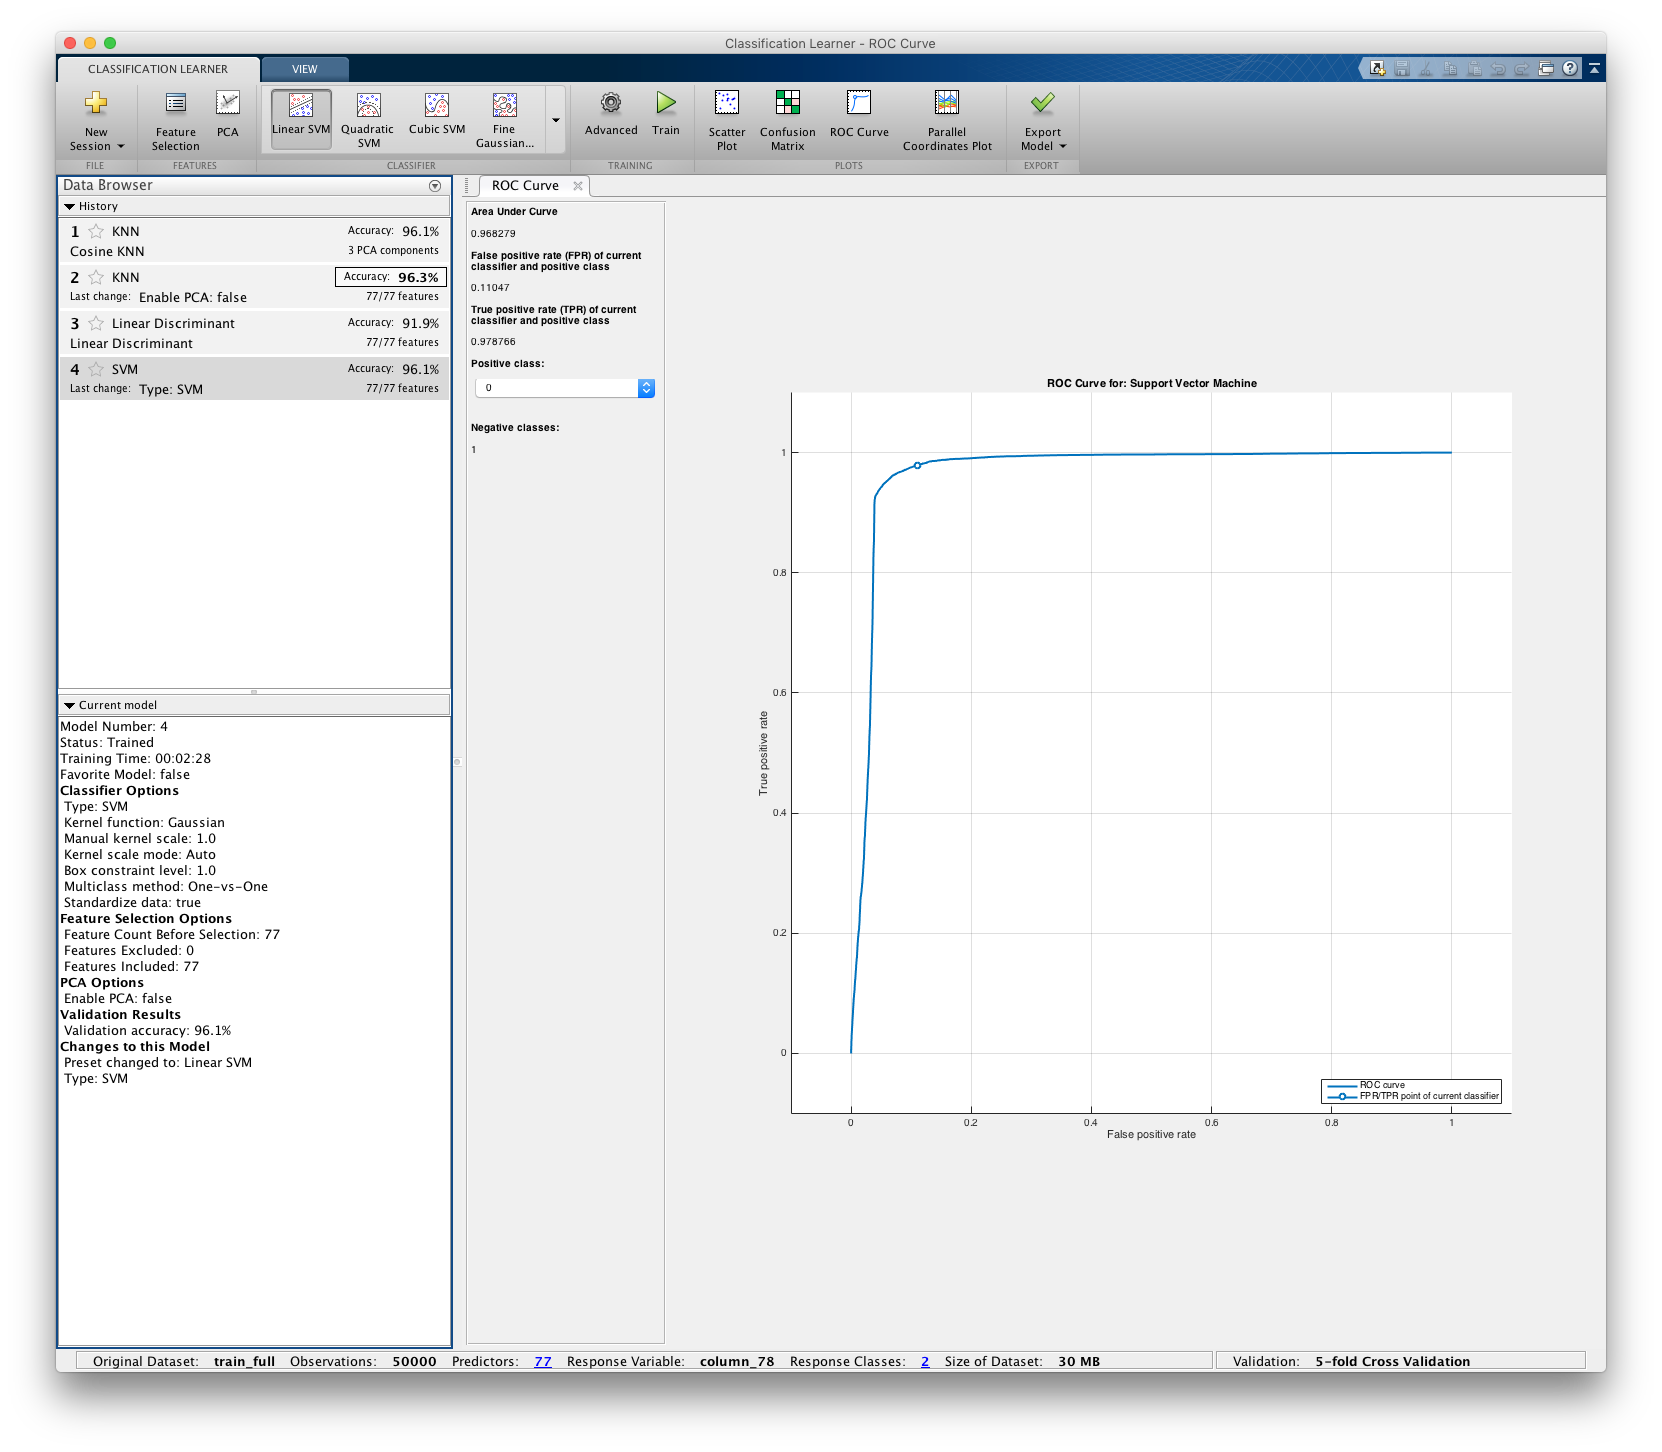
\includegraphics{matlab_train_m4}
	\caption{Fourth model: SVM (Gaussian kernel). }
	\label{fig:svm}
\end{figure*}

Finally deploy and predict. Save the models into Matlab workspace and predict labels for test (evaluation) dataset. Results are not shown here because these are not final submitted results. 

\bibliography{bib/yy1533_refs}
\bibliographystyle{plainnat}
\end{document}
